\section{Results}

\subsection{Joined TCGA+METABRIC training increased the effective sample size}

The final training design increased the available labeled training/validation pool from the TCGA-only setting to a joined TCGA+METABRIC setting. The joined pool contained 2737 samples, of which 2326 were used for training and 411 for validation. This directly addressed the main limitation observed in earlier TCGA-only neural experiments, where fewer than 700 training samples were available for models with tens of thousands of trainable parameters.

The parameter-count reduction experiment confirmed that the original Liquid/CfC model was moderately sized rather than extremely large. In the mRNA-only setting, the original Liquid/CfC model had 52,613 trainable parameters, whereas small-Liquid/CfC had 14,789. In the multimodal setting, the original Liquid/CfC model had 63,749 parameters, whereas small-Liquid/CfC had 20,357.

\subsection{External validation after adding METABRIC to training}

Adding METABRIC increased the training pool substantially and improved the competitiveness of Liquid/CfC on external cohorts. CPTAC 2020 was the most relevant multimodal external validation cohort because mRNA, CNA, and mutation features were all available. In the initial joined-training comparison, multimodal Liquid/CfC achieved the highest macro F1 among the tested Liquid, MLP, tree, and logistic models, narrowly outperforming mRNA-only MLP. This finding was subsequently reinterpreted after the extended baseline study, where elastic-net logistic regression and sklearn MLP slightly exceeded Liquid/CfC.

\begin{table}[ht]
\centering
\caption{CPTAC 2020 external validation.}
\begin{tabular}{llrr}
\toprule
Model & Feature set & Macro F1 & Macro ROC-AUC \\
\midrule
Liquid/CfC & Marker multimodal & 0.8806 & 0.9933 \\
MLP & Marker mRNA & 0.8803 & 0.9945 \\
small-Liquid/CfC & Marker multimodal & 0.8733 & 0.9927 \\
small-Liquid/CfC & Marker mRNA & 0.8676 & 0.9942 \\
Logistic regression & Marker mRNA & 0.8627 & 0.9878 \\
Liquid/CfC & Marker mRNA & 0.8584 & 0.9901 \\
ExtraTrees & Marker mRNA & 0.8247 & 0.9880 \\
MLP & Marker multimodal & 0.8188 & 0.9821 \\
\bottomrule
\end{tabular}
\label{tab:cptac}
\end{table}

\begin{figure}[ht]
\centering
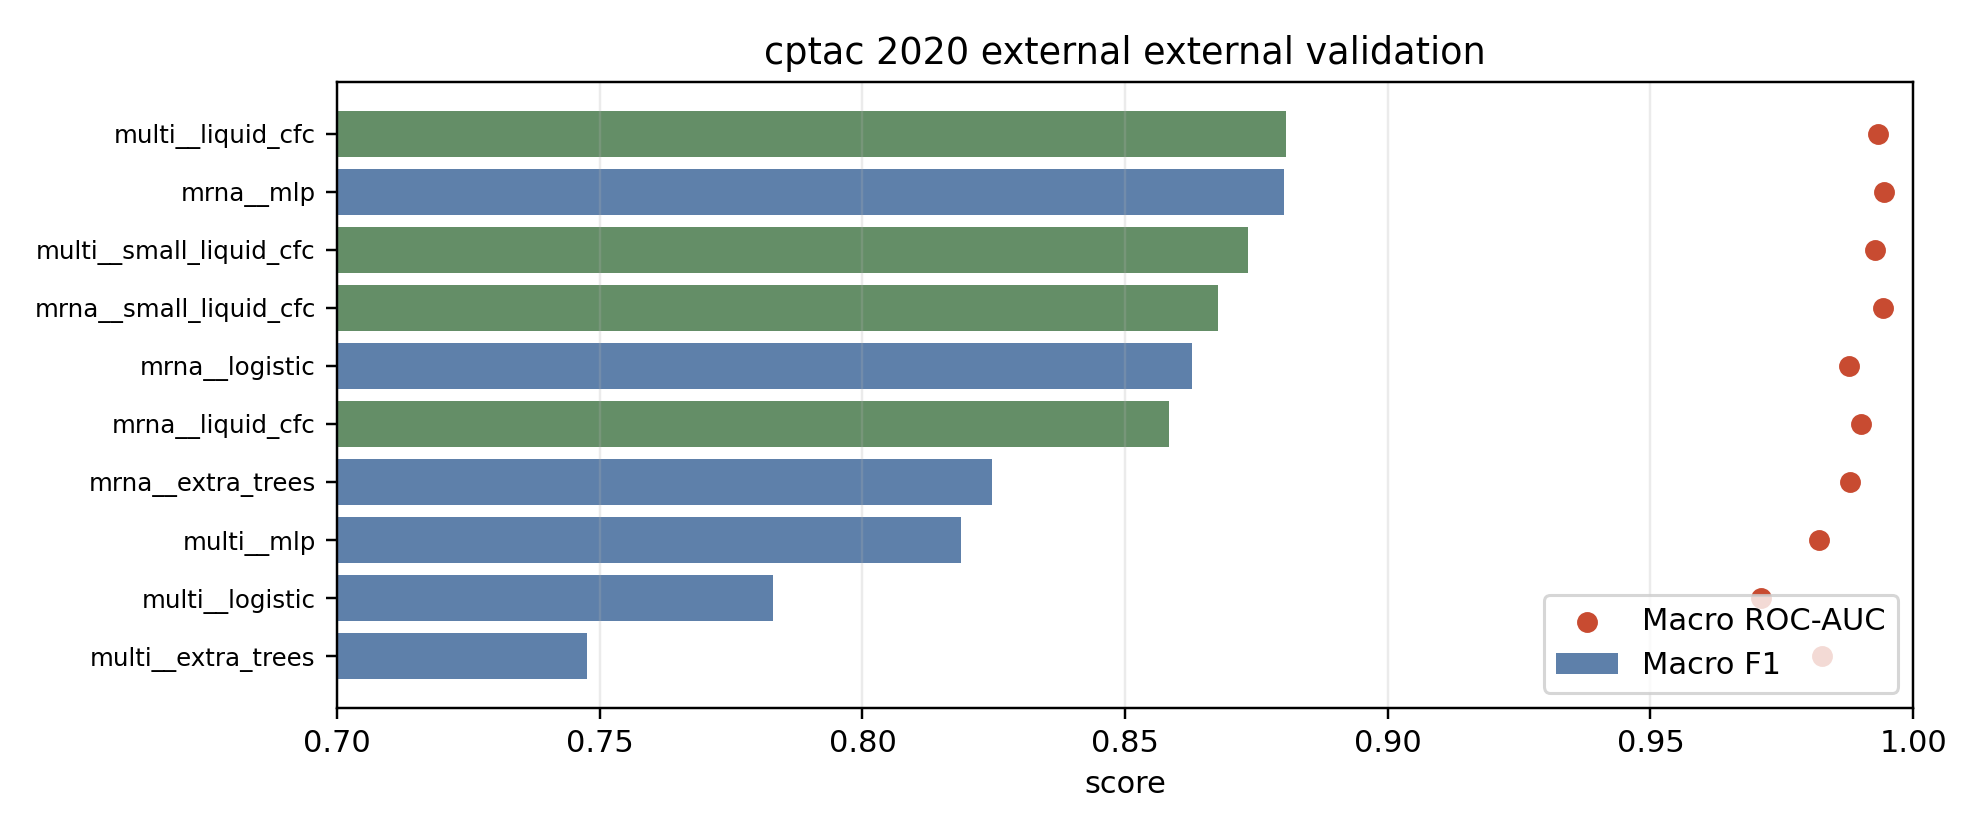
\includegraphics[width=0.85\linewidth]{figures/joined_small_liquid_cptac_2020_external_comparison.png}
\caption{CPTAC 2020 external validation after joined TCGA+METABRIC training.}
\label{fig:cptac}
\end{figure}

\subsection{mRNA-only external validation}

SMC 2018 and SCAN-B were used as mRNA marker external validation cohorts. These cohorts tested cross-cohort transfer of expression-marker models but could not directly evaluate complete multimodal fusion. In SCAN-B, the largest external cohort, ExtraTrees achieved the highest macro F1 (0.8493), followed by Liquid/CfC (0.8172). In SMC 2018, ExtraTrees was also the highest-scoring model (macro F1 = 0.9124), while Liquid/CfC was the strongest neural model (macro F1 = 0.8178).

These results show that strong expression-marker baselines remain difficult to beat when only mRNA features are available. They also indicate that Liquid/CfC is not simply superior by model class; its strongest result emerged in the multimodal CPTAC setting rather than in all expression-only transfers.

\begin{table}[ht]
\centering
\caption{mRNA marker external validation on SCAN-B and SMC 2018.}
\begin{tabular}{llrr}
\toprule
External cohort & Model & Macro F1 & Macro ROC-AUC \\
\midrule
SCAN-B & ExtraTrees & 0.8493 & 0.9831 \\
SCAN-B & Liquid/CfC & 0.8172 & 0.9830 \\
SCAN-B & MLP & 0.8033 & 0.9847 \\
SCAN-B & small-Liquid/CfC & 0.7857 & 0.9818 \\
SCAN-B & Logistic regression & 0.7851 & 0.9801 \\
\midrule
SMC 2018 & ExtraTrees & 0.9124 & 0.9894 \\
SMC 2018 & Liquid/CfC & 0.8178 & 0.9854 \\
SMC 2018 & small-Liquid/CfC & 0.7948 & 0.9838 \\
SMC 2018 & MLP & 0.7799 & 0.9840 \\
SMC 2018 & Logistic regression & 0.7751 & 0.9858 \\
\bottomrule
\end{tabular}
\label{tab:mrna_external}
\end{table}

\begin{figure}[ht]
\centering
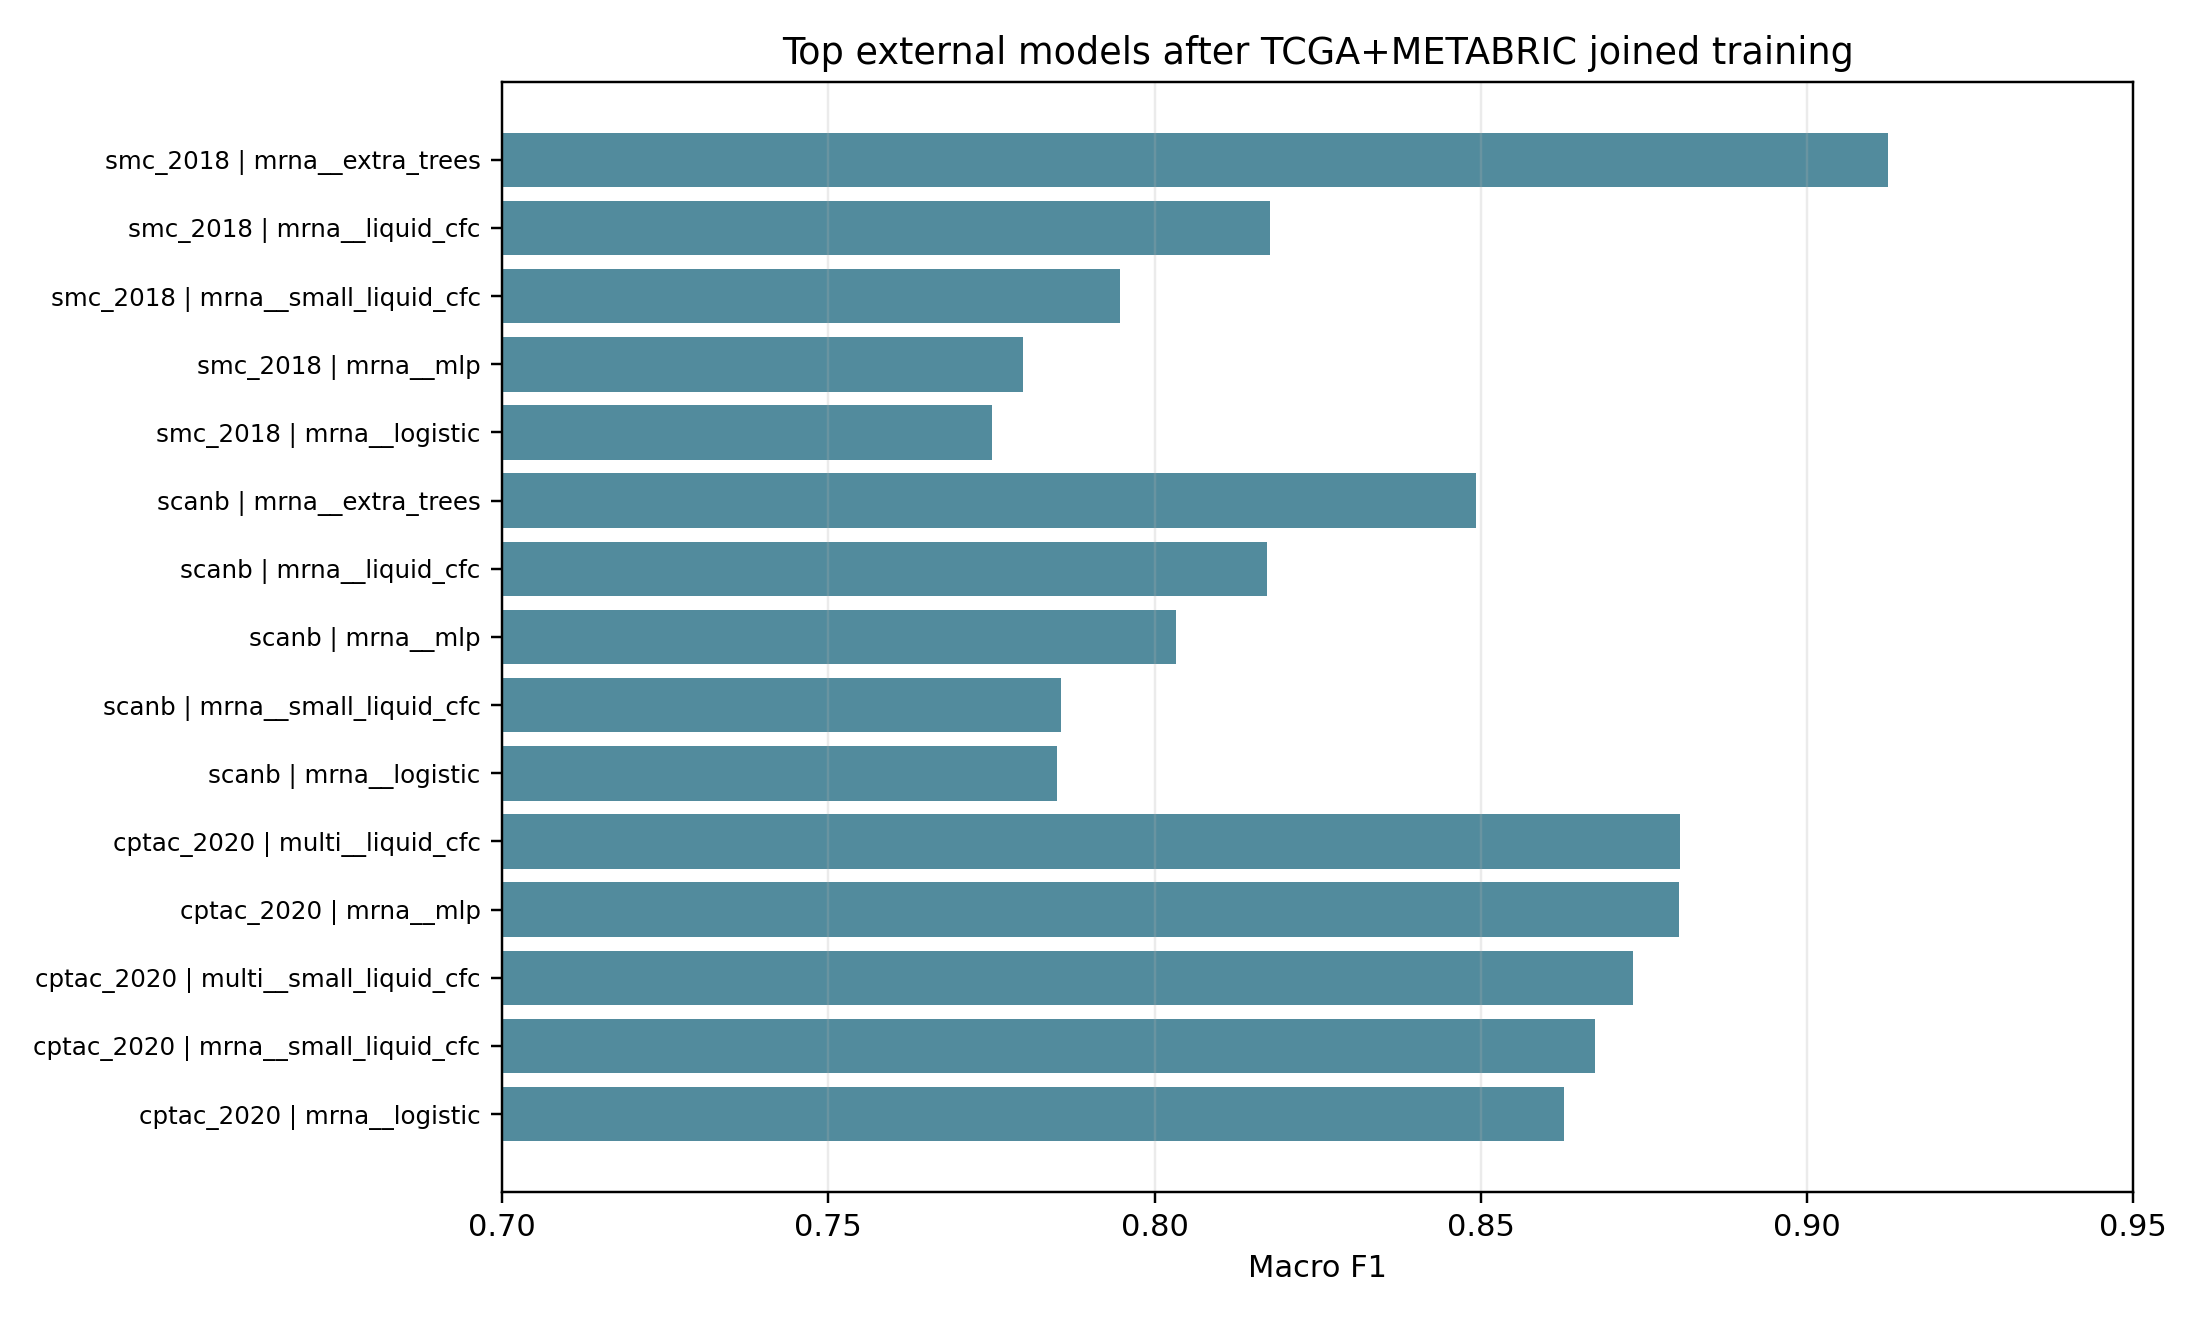
\includegraphics[width=0.9\linewidth]{figures/joined_small_liquid_top_external_macro_f1.png}
\caption{Top external models across CPTAC 2020, SMC 2018, and SCAN-B.}
\label{fig:top_external}
\end{figure}

\subsection{Effect of model-size reduction}

The small-Liquid/CfC model reduced the number of trainable parameters by approximately 68--72\% relative to the original Liquid/CfC model. Despite this reduction, small-Liquid/CfC did not consistently outperform the original model. On CPTAC 2020 multimodal validation, small-Liquid/CfC reached macro F1 of 0.8733, close to but below the original Liquid/CfC score of 0.8806. On SCAN-B and SMC 2018, small-Liquid/CfC was also below the original Liquid/CfC.

Therefore, reducing capacity alone did not solve cross-cohort generalization. The original Liquid/CfC model appeared to have enough capacity to benefit from the enlarged TCGA+METABRIC training pool, whereas the smaller model traded off parameter efficiency for slightly weaker external performance.

\subsection{Extended baseline study and expanded mRNA training scale}

We next expanded the baseline study to include elastic-net logistic regression, calibrated linear SVM, ridge classifier, shrinkage LDA, Gaussian Naive Bayes, k-nearest neighbors, random forest, ExtraTrees, histogram gradient boosting, and an sklearn MLP. This analysis was performed in the mRNA marker setting because SCAN-B and SMC 2018 did not provide the complete CNA and mutation feature set required for clean multimodal training.

Two training scales were compared. The first used the joined TCGA+METABRIC training pool. The second further added SCAN-B and SMC 2018 to create an expanded mRNA training pool, while keeping CPTAC 2020 as the independent external validation cohort. Contrary to a simple sample-size expectation, the expanded mRNA training pool did not improve the best CPTAC external macro F1. Elastic-net logistic regression and sklearn MLP trained on TCGA+METABRIC slightly exceeded multimodal Liquid/CfC on CPTAC macro F1, although the differences were small.

\begin{table}[ht]
\centering
\caption{CPTAC external comparison after extended baseline analysis.}
\resizebox{\textwidth}{!}{%
\begin{tabular}{lllrr}
\toprule
Training scale & Model & Feature set & Macro F1 & Macro ROC-AUC \\
\midrule
TCGA+METABRIC & Logistic ElasticNet & mRNA marker & 0.8830 & 0.9899 \\
TCGA+METABRIC & sklearn MLP & mRNA marker & 0.8823 & 0.9940 \\
TCGA+METABRIC & Liquid/CfC & multimodal marker & 0.8806 & 0.9933 \\
TCGA+METABRIC & MLP & mRNA marker & 0.8803 & 0.9945 \\
TCGA+METABRIC & small-Liquid/CfC & multimodal marker & 0.8733 & 0.9927 \\
Expanded mRNA & sklearn MLP & mRNA marker & 0.8559 & 0.9940 \\
Expanded mRNA & Logistic ElasticNet & mRNA marker & 0.8509 & 0.9911 \\
Expanded mRNA & HistGradientBoosting & mRNA marker & 0.8443 & 0.9869 \\
\bottomrule
\end{tabular}
}
\label{tab:extended_baselines}
\end{table}

\begin{figure}[ht]
\centering
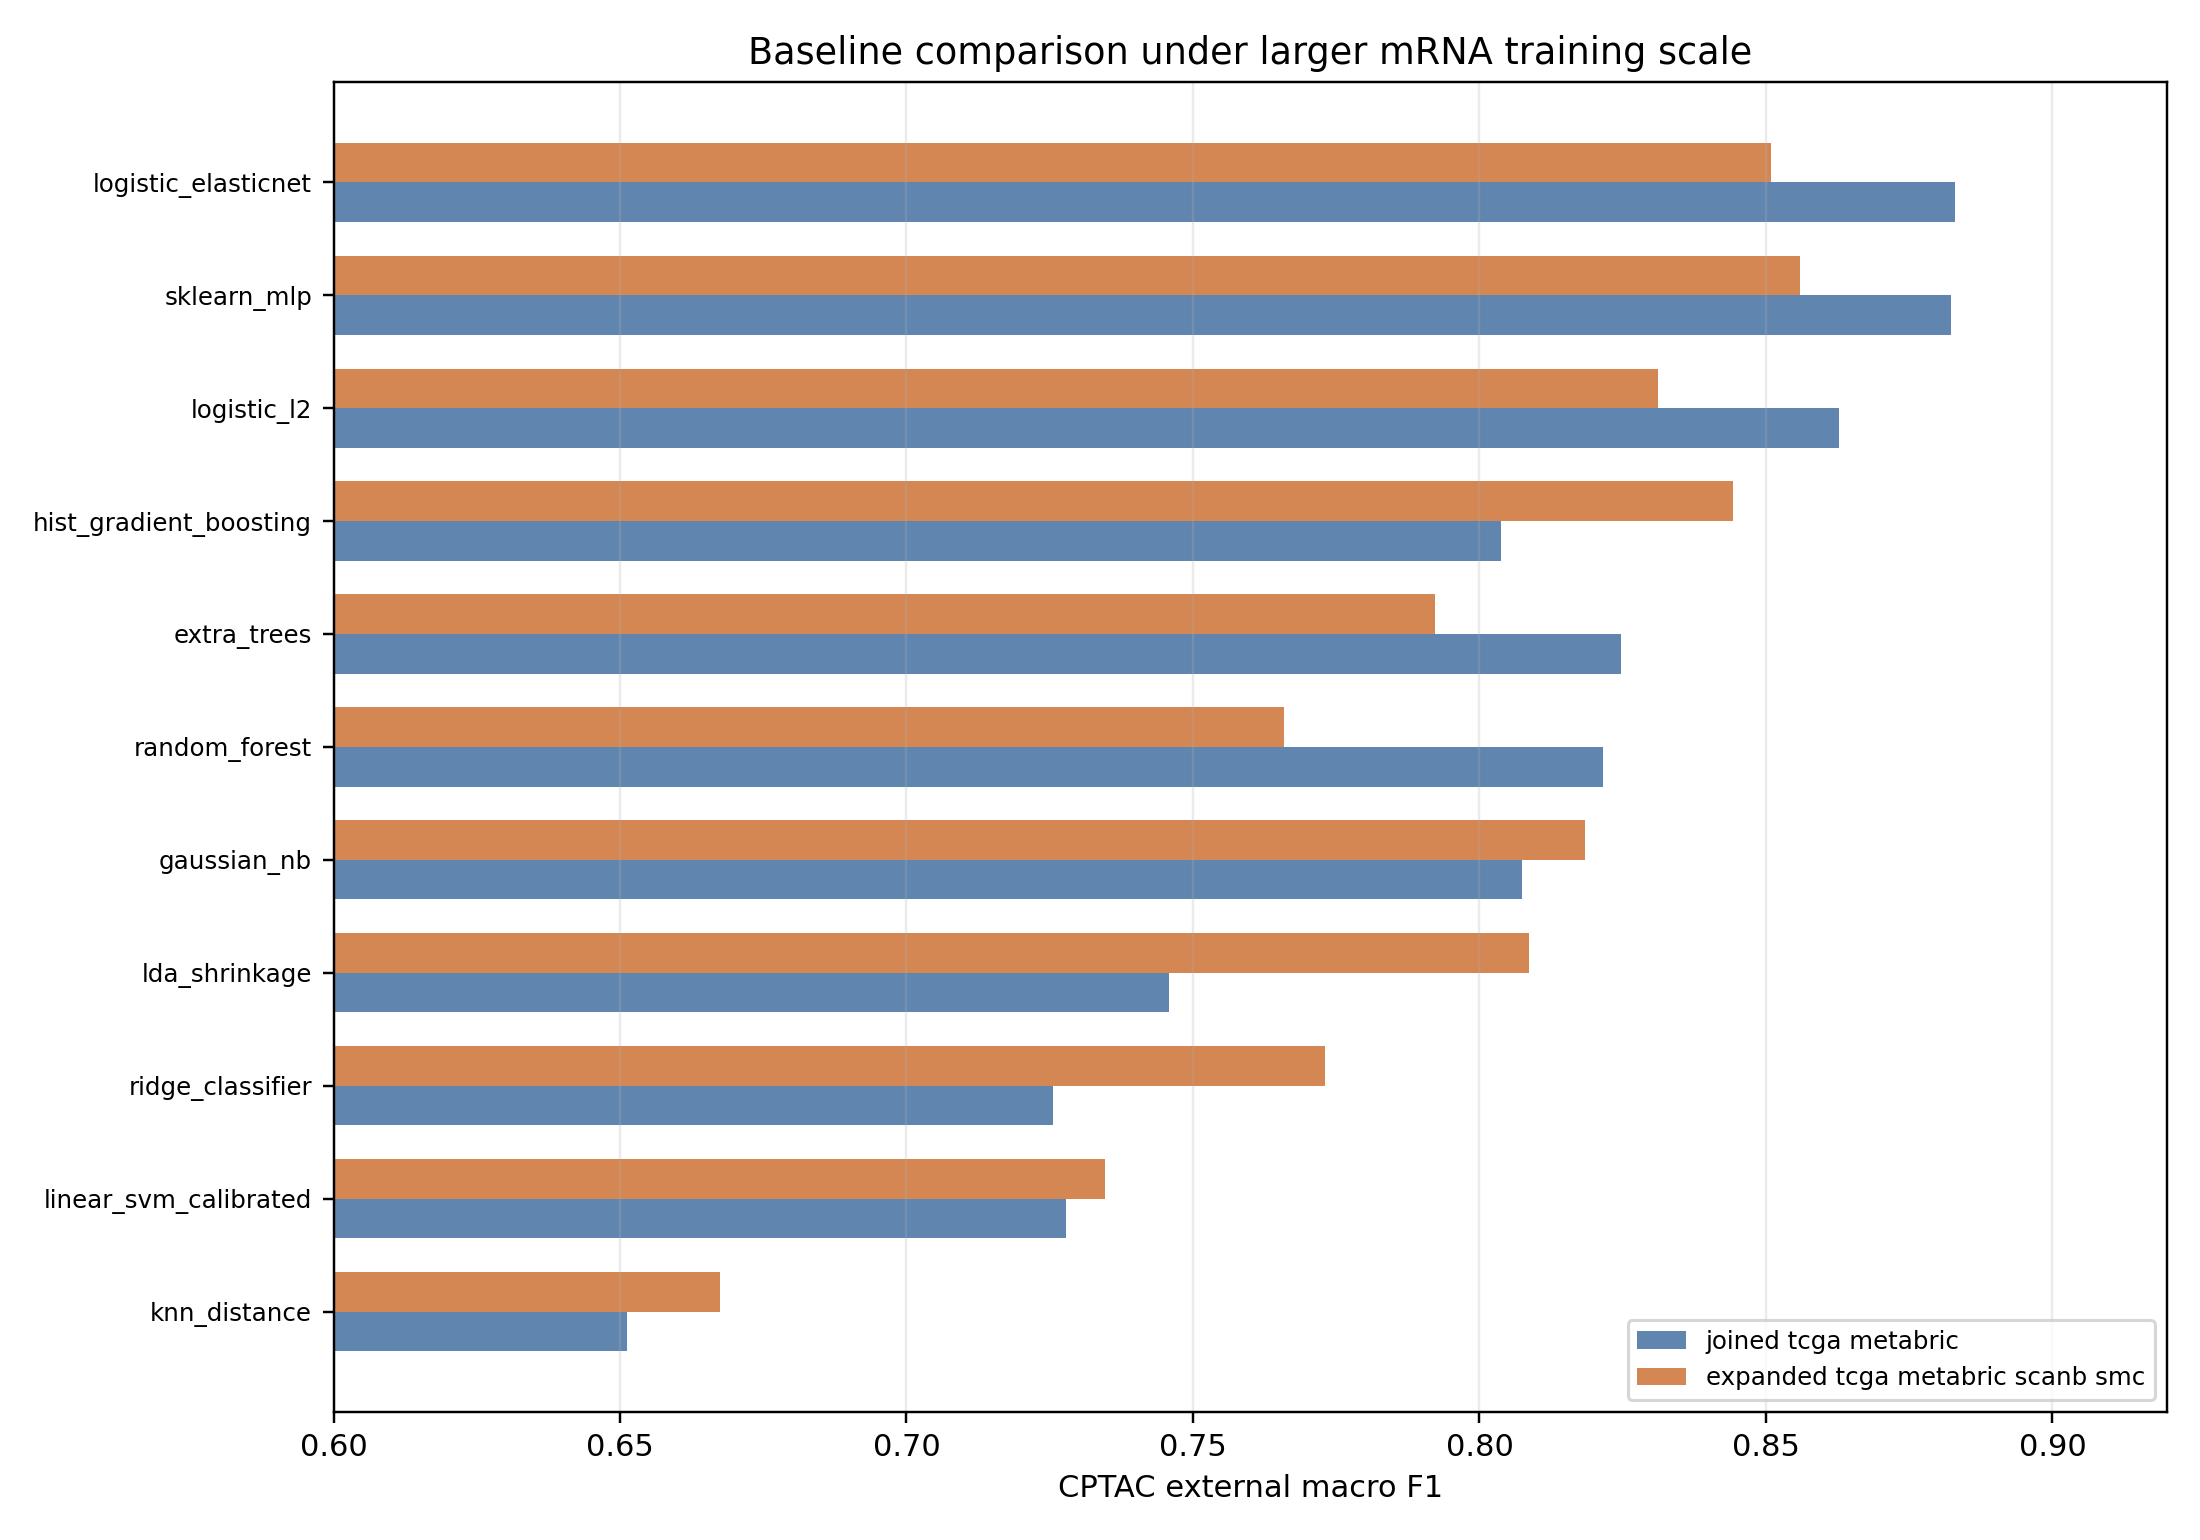
\includegraphics[width=0.9\linewidth]{figures/large_scale_mrna_baseline_cptac_f1.png}
\caption{CPTAC external macro F1 for extended mRNA baselines under TCGA+METABRIC training and expanded TCGA+METABRIC+SCAN-B+SMC training.}
\label{fig:large_baselines}
\end{figure}

\begin{figure}[ht]
\centering
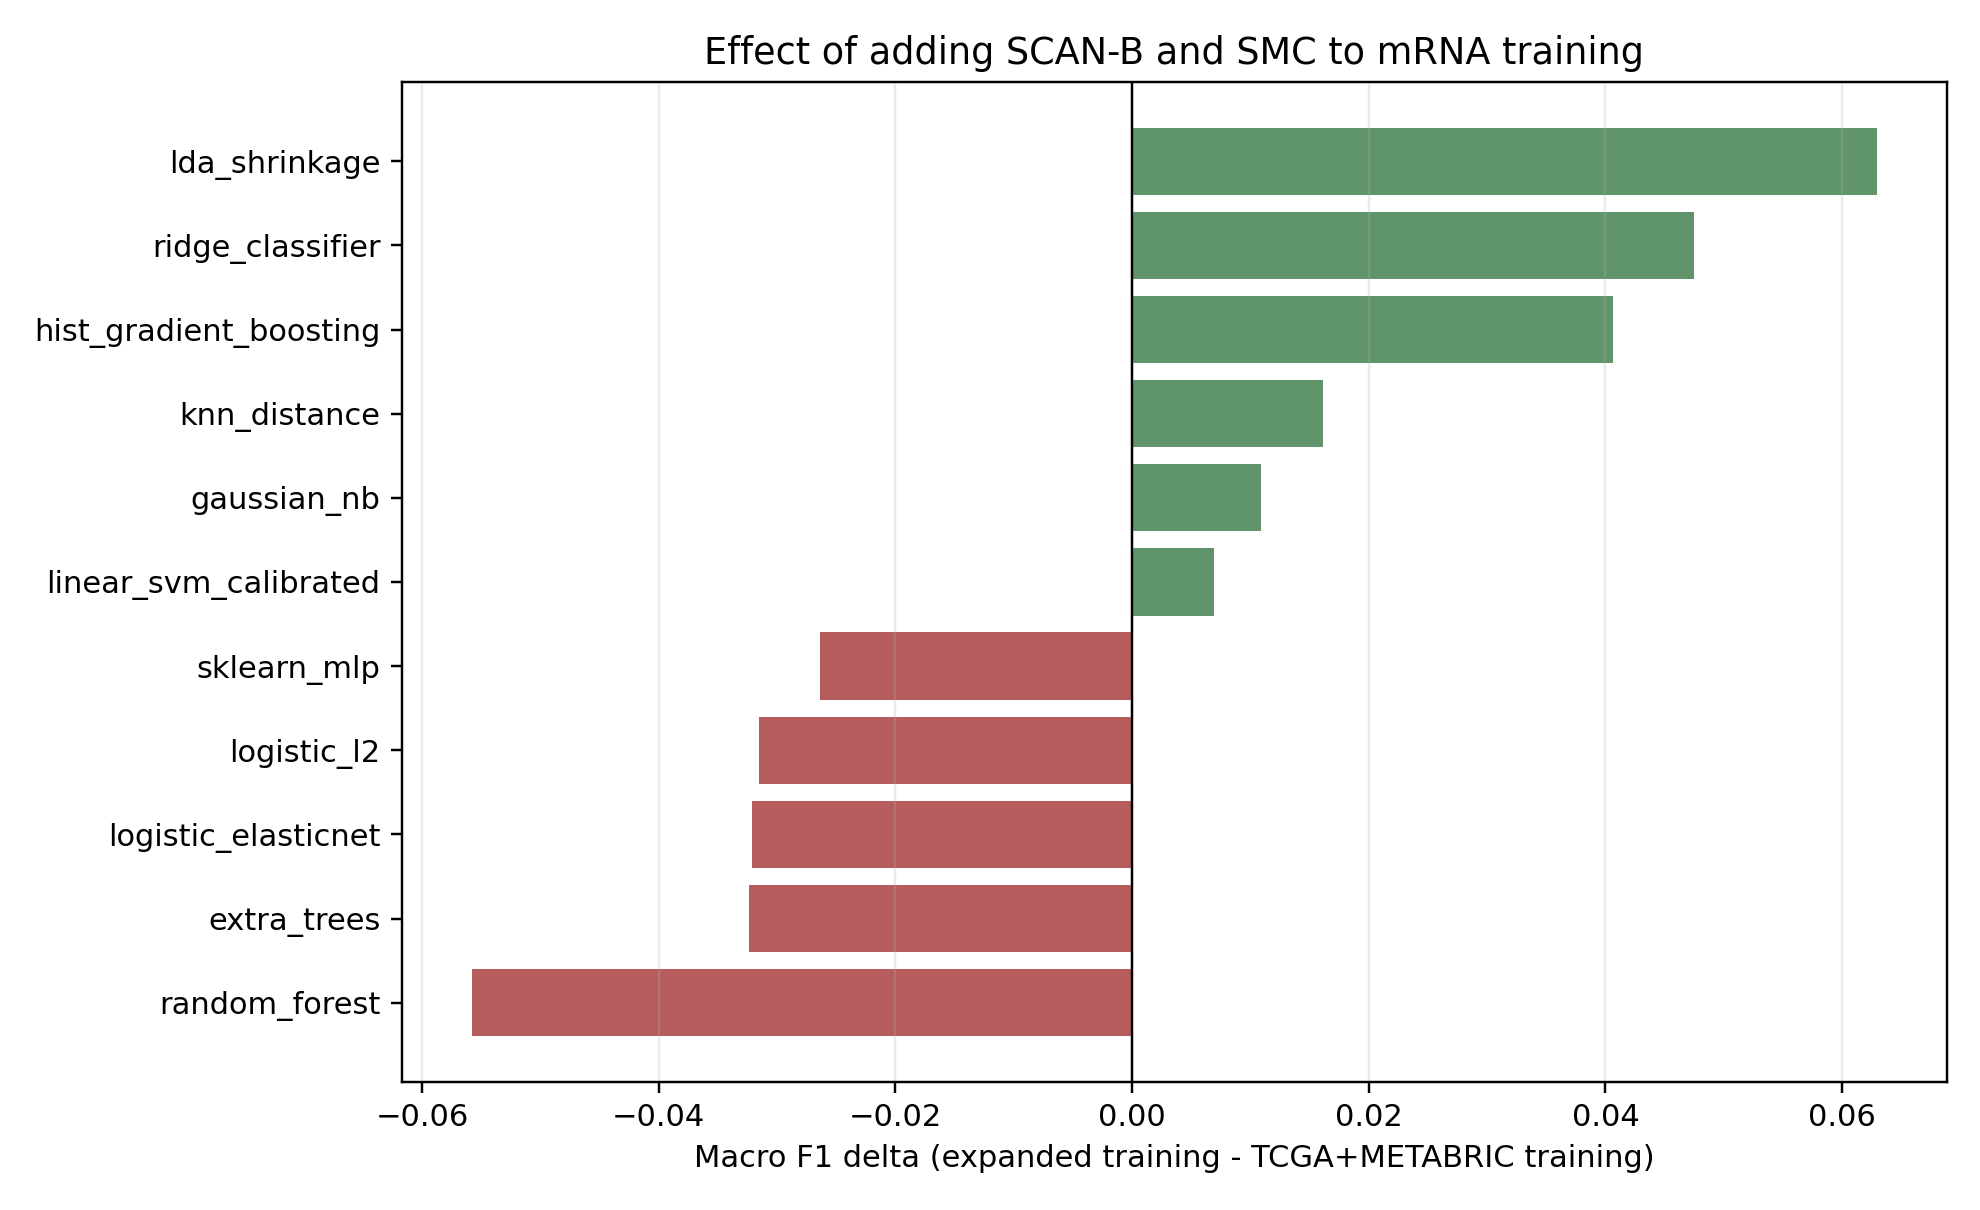
\includegraphics[width=0.85\linewidth]{figures/large_scale_mrna_training_delta_cptac_f1.png}
\caption{Change in CPTAC external macro F1 after adding SCAN-B and SMC 2018 to the mRNA training pool. Negative values indicate reduced external performance after training-scale expansion.}
\label{fig:training_delta}
\end{figure}

\subsection{Multi-cancer internal benchmark}

To move beyond a single-cancer benchmark, we added five cancer-internal prediction tasks from TCGA PanCancer Atlas cohorts. The tasks differed in difficulty. UCEC molecular subtype, COADREAD molecular subtype, and HNSC HPV status were highly predictable, whereas KIRC grade and PRAD pathologic T stage were substantially harder.

No model was best across all tasks. ExtraTrees was strongest for COADREAD molecular subtype and HNSC HPV status. Elastic-net logistic regression was strongest for UCEC molecular subtype. Histogram gradient boosting achieved the highest macro F1 for KIRC grade. small-Liquid/CfC achieved the highest macro F1 for PRAD pathologic T-stage prediction. Complete task-specific model results and label distributions are provided in Supplementary Tables~\ref{tab:supp_label_counts}--\ref{tab:supp_prad}. A core-aligned sensitivity analysis excluding sparse RPPA features is reported in Supplementary Table~\ref{tab:supp_core_aligned}; in that setting, Liquid/CfC was best for COADREAD molecular subtype, whereas other tasks were still led by linear, tree, or boosting baselines. This task-dependent ranking supports the interpretation that Liquid/CfC is a context-dependent fusion candidate rather than a universal winner.

\begin{table}[ht]
\centering
\caption{Best model for each cancer-internal benchmark task.}
\begin{tabular}{llrr}
\toprule
Task & Best model & Macro F1 & Macro ROC-AUC \\
\midrule
HNSC HPV status & ExtraTrees & 0.9505 & 0.9942 \\
UCEC molecular subtype & Logistic ElasticNet & 0.9134 & 0.9831 \\
COADREAD molecular subtype & ExtraTrees & 0.9060 & 0.9546 \\
PRAD pathologic T stage & small-Liquid/CfC & 0.7071 & 0.7717 \\
KIRC grade & HistGradientBoosting & 0.6996 & 0.7556 \\
\bottomrule
\end{tabular}
\label{tab:multicancer_best}
\end{table}

\begin{figure}[ht]
\centering
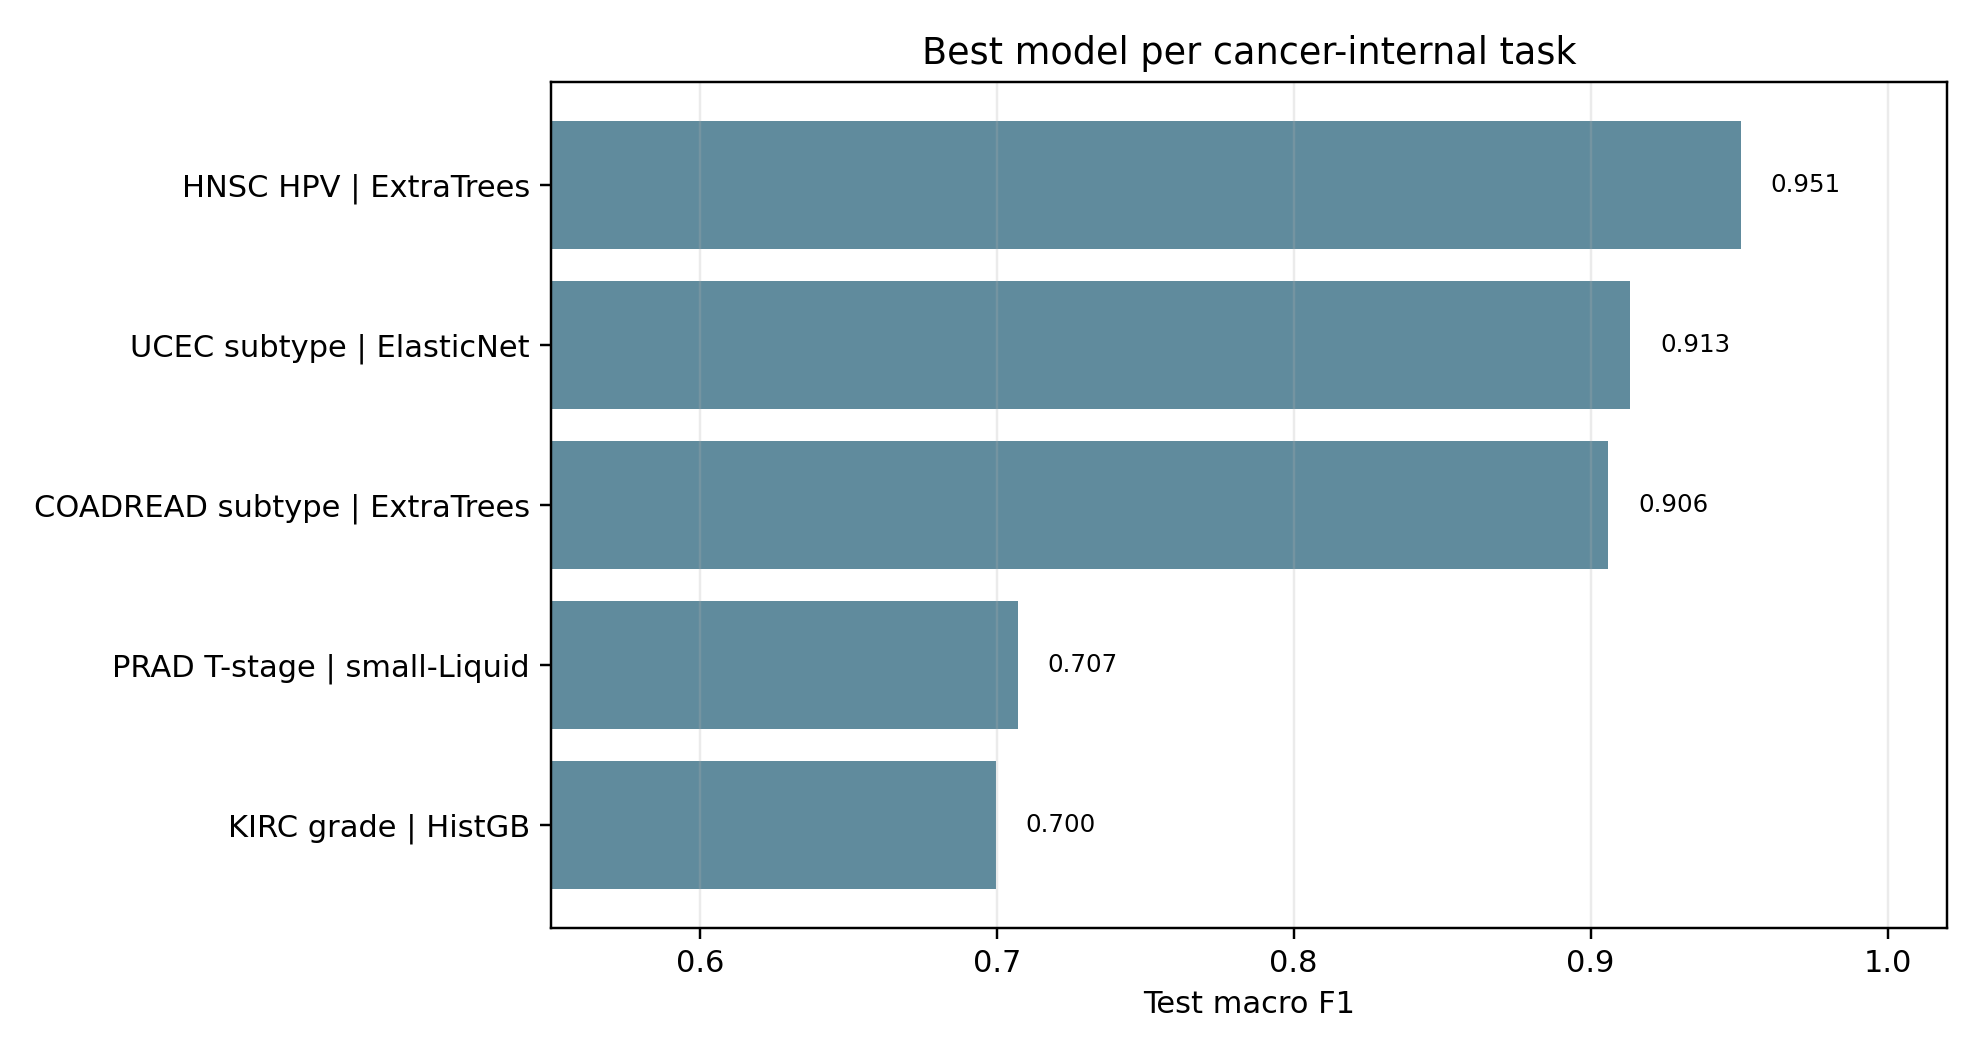
\includegraphics[width=0.85\linewidth]{figures/multicancer_internal_best_by_task.png}
\caption{Best model per cancer-internal benchmark task.}
\label{fig:multicancer_best}
\end{figure}

\begin{figure}[ht]
\centering
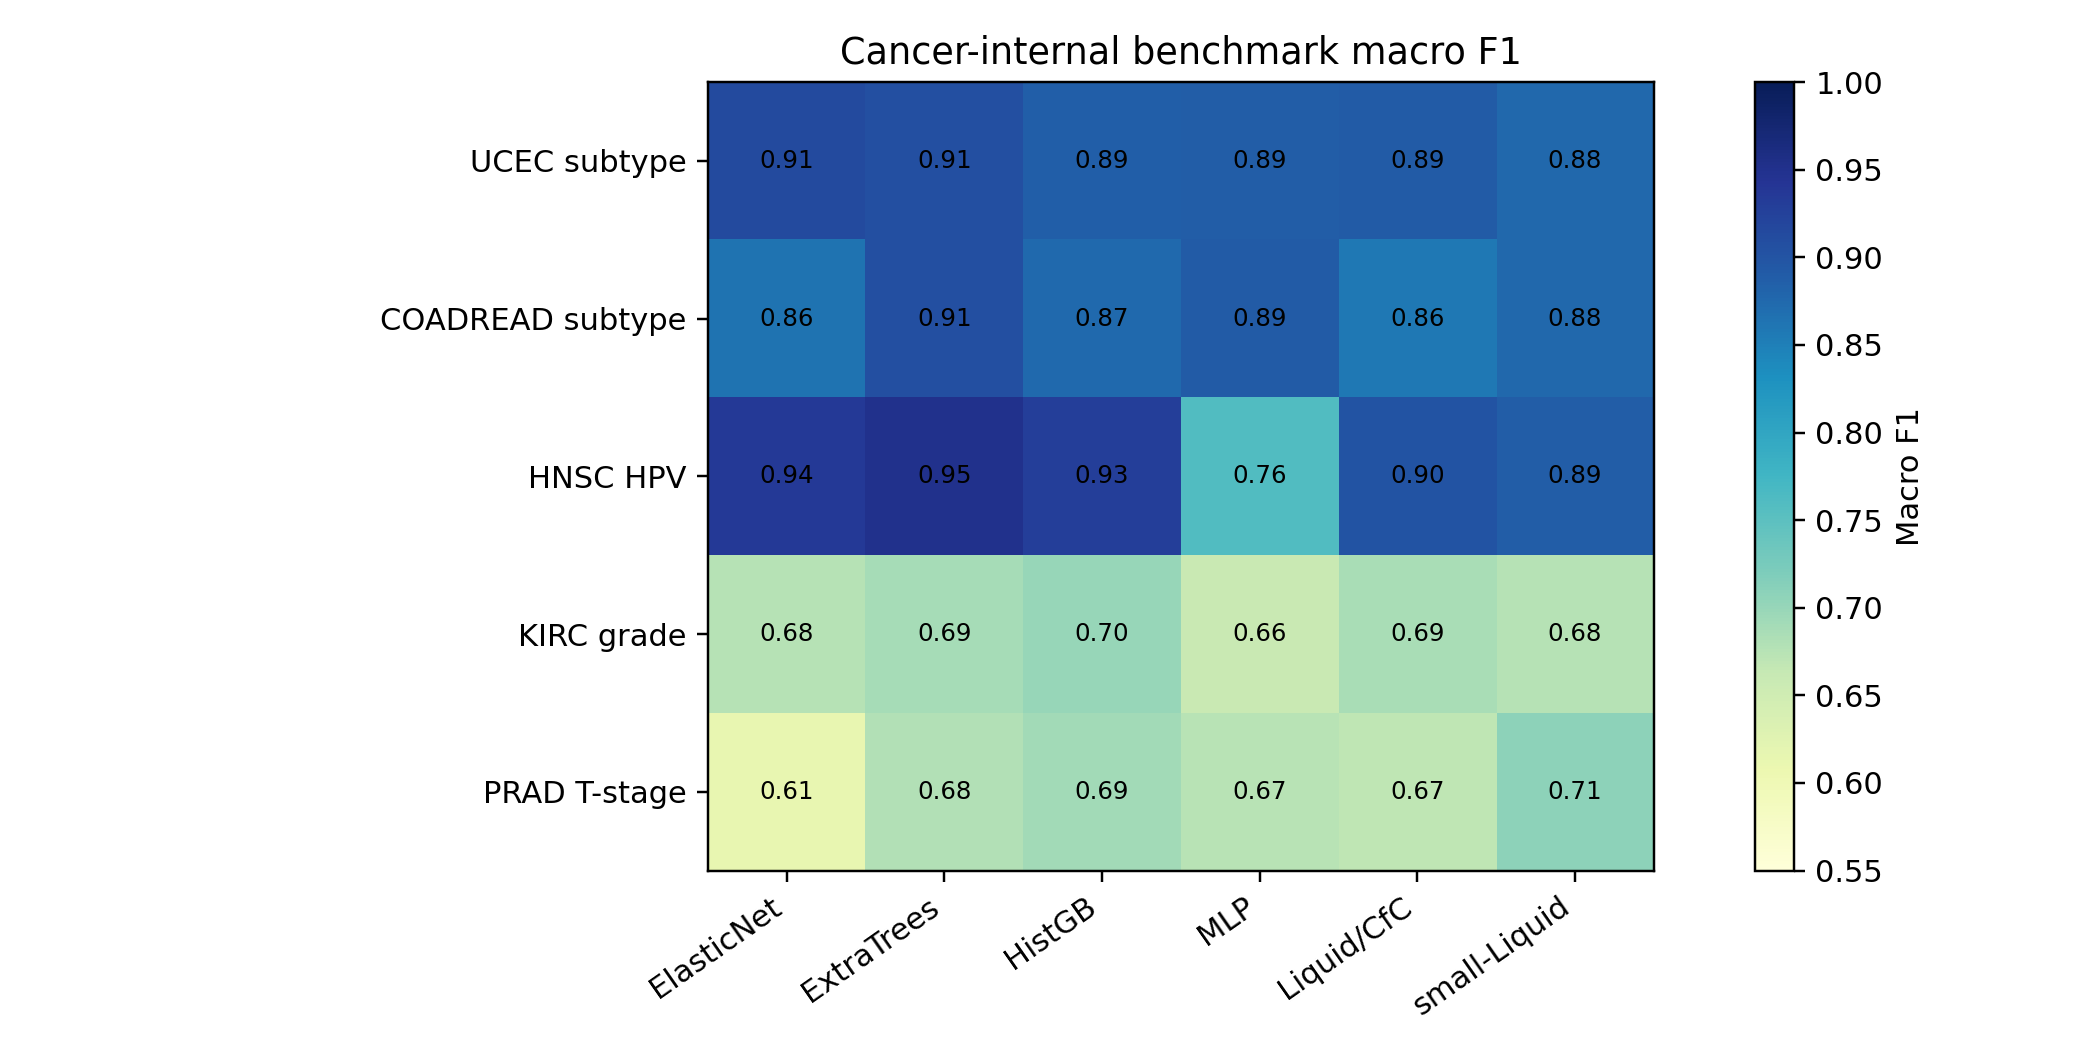
\includegraphics[width=0.95\linewidth]{figures/multicancer_internal_model_task_heatmap.png}
\caption{Macro F1 across models and cancer-internal tasks. The heatmap shows that model ranking is strongly task-dependent.}
\label{fig:multicancer_heatmap}
\end{figure}

\subsection{Cross-validation, significance, and noise robustness}

The ten-fold core-aligned cross-validation analysis confirmed that model ranking varied by task. ExtraTrees was highest for COADREAD molecular subtype (macro F1 = 0.8676), KIRC grade (0.6662), and UCEC molecular subtype (0.8944); logistic ElasticNet was highest for HNSC HPV status (0.9469); and histogram gradient boosting was highest for PRAD pathologic T stage (0.6818). However, none of the top-versus-runner-up paired fold-level comparisons was statistically significant. The paired macro F1 differences were small, ranging from 0.0036 to 0.0159, all bootstrap confidence intervals crossed zero, and the minimum unadjusted paired-test \(p\)-value was 0.375 (Supplementary Table~\ref{tab:supp_cv_significance}). No comparison survived Holm correction across the five tasks. We therefore interpret the task-level rankings as descriptive rather than as evidence of statistically significant universal superiority.

Noise robustness analysis also supported a cautious interpretation. For the best cross-validated model in each task, performance under moderate test-time Gaussian noise was generally stable for HNSC and UCEC but degraded more clearly for COADREAD, KIRC, and PRAD. The estimated noise elbows occurred around \(\sigma=0.30\) for COADREAD, HNSC, KIRC, and UCEC, and around \(\sigma=0.10\) for PRAD (Supplementary Table~\ref{tab:supp_noise_elbow}). PRAD reached a 5\% macro F1 drop by \(\sigma=0.10\), KIRC by \(\sigma=0.20\), and COADREAD by \(\sigma=0.30\), whereas HNSC and UCEC did not reach a 5\% drop by \(\sigma=0.50\). This suggests that some apparent score differences may indeed be within the scale of fold-to-fold and perturbation-level variability.

\subsection{Summary of empirical findings}

The final empirical pattern was cohort- and task-dependent. When aligned multimodal external data were available, as in CPTAC 2020, multimodal Liquid/CfC was highly competitive. However, after strengthening the baseline suite, elastic-net logistic regression and MLP slightly exceeded Liquid/CfC on CPTAC macro F1. On larger mRNA-only external cohorts, expression-marker models and tree-based baselines remained very strong. In the multi-cancer internal benchmark, different model families were optimal for different endpoints. Ten-fold CV and noise analysis further showed that many top-rank differences were small and not statistically significant. Therefore, the evidence supports Liquid/CfC as a useful cross-omics fusion candidate, rather than a universally dominant cancer multi-omics classifier.
